%\documentclass[t,14pt,serif,professionalfonts,mathtt]{beamer}
\documentclass[10pt,t]{beamer}

\usepackage[utf8]{inputenc}
\usepackage[english,russian]{babel}

\usepackage{amssymb,amsfonts,amsmath,mathtext}
\usepackage{cite,enumerate,float,indentfirst}
\usepackage{graphicx}
\usepackage{epstopdf}
\epstopdfsetup{suffix=}

\usepackage{setspace}



\usepackage{tikz}

%\usetheme{Warsaw}
%\usetheme{Berkeley}
%\usetheme{Rochester}
%\usetheme{Malmoe}
\usetheme{Darmstadt}

\usefonttheme[onlymath]{serif}

\setbeamertemplate{headline}{}

\setbeamertemplate{footline}
{%
\begin{beamercolorbox}{section in head/foot}
  \vskip2pt%
  \hbox to \paperwidth{\insertnavigation{0.95\paperwidth} \hfill% 
    {\scriptsize \bfseries \insertframenumber}\hspace*{3mm}}%
  \vskip2pt
\end{beamercolorbox}%
}

\setcounter{tocdepth}{1}

\newtheorem{defin}{Определение}
\newtheorem{theo}{Теорема}

%%%%%%%%%%%%%%%%%%%%%%%%%%%%%%%%%%%%%%%%%%%%%%%%%%%%%%%

\newcommand{\mathbi}[1]{\text{\rmfamily \textit{\textbf{#1}}}}

\newcommand{\ts}{\mathcal T}
\newcommand{\fs}{\mathcal F}
\newcommand{\gs}{\mathcal G}
\newcommand{\Lgr}{{\mathcal L}}
\newcommand{\Mm}{\mathcal M}
\newcommand{\ve}{\varepsilon}

\DeclareMathOperator{\Var}{Var}
\DeclareMathOperator{\interior}{int}
\DeclareMathOperator{\cl}{cl}
\DeclareMathOperator{\co}{co}
\DeclareMathOperator{\conv}{conv}
\DeclareMathOperator{\dist}{dist}
\DeclareMathOperator{\gr}{gr}
\DeclareMathOperator{\epi}{epi}
\DeclareMathOperator{\hypo}{hypo}

%\newtheorem{defin}{Определение}
%\newtheorem{theo}{Tеорема}
%\newtheorem{proposition}{Предложение}
%\newtheorem{consequence}{Следствие}
%\newtheorem{lemma}{Лемма}

\makeatletter 
\def\myitem#1{\item[#1] \def\@currentlabel{#1}} 
\makeatother
%%%%%%%%%%%%%%%%%%%%%%%%%%%%%%%%%%%%%%%%%%%%%%%%%%%%%%%
\begin{document}

\definecolor{navyBlue}{RGB}{0,51,153}
\definecolor{deepBlue}{RGB}{51,0,204}
\definecolor{forestGreen}{RGB}{0,102,51}

\setbeamertemplate{footline}{}

\setbeamertemplate{blocks}[rounded][shadow=false]

\setbeamercolor*{normal text}{fg=navyBlue}
\usebeamercolor[fg]{normal text}

\setbeamercolor*{math text}{fg=black}

\beamertemplatenavigationsymbolsempty
%--------------------------------------------------------------------------------
%% титульная страница
\definecolor{confColor}{RGB}{153,51,102}

\setbeamerfont{title}{shape=\itshape,family=\bfseries}

\setbeamerfont{author}{family=\itshape}
\setbeamercolor{author}{fg=forestGreen}

\setbeamerfont{institute}{family=\itshape}
\setbeamercolor{institute}{fg=forestGreen}

\setbeamerfont{date}{family=\bfseries, size=}
\setbeamercolor{date}{fg=confColor}

\title[Разработка программного комплекса моделирования и визуализации движения беспилотных летательных аппартов]{Разработка программного комплекса моделирования и визуализации движения беспилотных летательных аппаратов}

\author{Дербенев Леонид Олегович}

\institute{Институт математики и механики им. Н.Н.\,Красовского}

%\date{\small \bigskip

%47-я Всероссийская молодежная школа-конференция <<Современные проблемы математики и ее приложений>>\\

% 31 января -- 6 февраля 2016 г.}

%\vspace*{-10mm}

\maketitle


%--------------------------------------------------------------------------------
%% Outline
%\section{План}

\setbeamertemplate{footline}
{%
\begin{beamercolorbox}{section in head/foot}
  \vskip2pt%
  \hbox to \paperwidth{\insertnavigation{0.95\paperwidth} \hfill% 
    {\scriptsize \bfseries \insertframenumber}\hspace*{3mm}}%
  \vskip2pt
\end{beamercolorbox}%
}


%\begin{frame}
%
%\frametitle{План}
%
%\Large
%
%\tableofcontents
%
%\end{frame}
%--------------------------------------------------------------------------------

\section[Задача]{Задача}
\subsection[Задача]{Задача}
\begin{frame}
\frametitle{Задача}
\small



\end{frame}

%--------------------------------------------------------------------------------
\section[Модели движения]{Модели двжиения}
\subsection[Материальная точка]{Материальная точка}
\begin{frame}
\frametitle{Материальная точка}
\small

Материальная точка имеет следующую модель движения:
\begin{equation*}
    \Ddot{r} = m \cdot u,
\end{equation*}
где $r = (x, y, z)^\text{\textup{T}}$~--- радиус\=/вектор положения объекта, $u = (u_x, u_y, u_z)^\text{\textup{T}}$~--- управление, являющееся ускорением, $m$~--- масса точки.

Покоординатная запись:
\begin{equation*}
  \ddot{x} = u_x, \quad \ddot{y} = u_y, \quad \ddot{z} = u_z.
\end{equation*}

Запись, включающая скорости:
\begin{alignat*}{3}
  & \dot{x} = V_x,  & \quad & \dot{y} = V_y, & \quad & \dot{z} = V_z, \\
  & \dot{V_x} = u_x, & & \dot{V_y} = u_y, & & \dot{V_z} = u_z.
\end{alignat*}
\end{frame}

%--------------------------------------------------------------------------------
\subsection[Коптер]{Коптер}
\begin{frame}
\frametitle{Коптер}
\small

Коптер имеет следующую модель:
\begin{alignat*}{3}
  & \dot{x} = V_x, & \quad & \dot{y} = V_y, & \quad
    & \dot{z} = V_z, \\
  & \displaystyle
    \dot{V_x} = \frac{u_x - V_x}{l_{xz}},  & &
    \dot{V_y} = \frac{u_y - V_y}{l_{y}},   & &
    \dot{V_z} = \frac{u_z - V_y}{l_{xz}}.
\end{alignat*}
Здесь $u = (u_x, u_y, u_z)^\text{\textup{T}}$~--- управление, командный сигнал скорости, имеющий смысл желаемой скорости по каждой из координат; $l_{xz}$, $l_y$~--- коэффициенты, описывающие инерционность выхода на выбранный уровень скорости: выход осуществляется за время порядка $3l$. 
\end{frame}
%--------------------------------------------------------------------------------
\subsection[Вертолет]{Вертолет}
\begin{frame}
\frametitle{Вертолет}
\small

\begin{equation*}
  \begin{array}{l}
    \dot x = V_\text{гор} \cos \psi, \\[0.75ex]
    \dot z = V_\text{гор} \sin \psi, \\[0.75ex]
    \dot y = V_\text{верт}, \\[0.75ex]
    \dot \psi   = \frac{\beta_\text{бок}}{V_\text{гор}} \, u_\text{бок}, \quad |u_\text{бок}| \leqslant 1, \\[0.75ex]
    \dot V_\text{гор} = a, \quad  
      a_{\min} \leqslant a \leqslant a_{\max},
      \quad V^{\min}_\text{гор} \leqslant V_\text{гор} \leqslant V^{\min}_\text{гор}, \\[0.75ex]
    \dot V_\text{верт} = u_\text{верт},
      \quad u^{\min}_\text{верт} \leqslant u_\text{верт} \leqslant u^{\max}_\text{верт}, \quad
      V^{\min}_\text{верт} \leqslant V_\text{верт} \leqslant V^{\max}_\text{верт}.
  \end{array}
\end{equation*}

Здесь $\psi$~--- угол курса; $u_\text{бок}$~--- ускорение, управляющее разворотом круса; $u_\text{верт}$~--- ускорение (создаваемое изменением скорости вращения винтов), управляющее вертикальной скоростью; $a$~--- ускорение, управляющее величиной горизонтальной скорости (продольное); $\beta_\text{бок}$~--- коэффициент горизонтальной маневренности судна.

\end{frame}
%--------------------------------------------------------------------------------
\subsection[Самолет]{Самолет}
\begin{frame}
\frametitle{Самолет}
\small

\begin{equation*}
  \begin{array}{l}
    \dot x = V \cos \theta \cos \psi, \\[0.75ex]
    \dot z = V \cos \theta \sin \psi, \\[0.75ex]
    \dot y = V \sin \theta, \\[0.75ex]
    \dot \theta = \frac{\beta_\text{верт}}{V} \, u_\text{верт}, \\[0.75ex]
    \dot \psi   = \frac{\beta_\text{бок}}{V} \, u_\text{бок}, \\[0.75ex]
    |u_\text{верт}| \leqslant 1, 
      \quad |u_\text{бок}| \leqslant 1, \\[0.75ex]
    \dot V = a, \quad  
      a_{\min} \leqslant a \leqslant a_{\max},
      \quad V_{\min} \leqslant V \leqslant V_{\max}.
  \end{array}
\end{equation*}

Здесь $\theta$~--- угол тангажа, $\psi$~--- угол курса; $u_\text{верт}$, $u_\text{бок}$~--- ускорения, управляющие углами тангажа и курса; $a$~--- ускорение, управляющее скоростью; $\beta_\text{верт}$, $\beta_\text{бок}$~--- коэффициенты маневренности судна. 

\end{frame}
%--------------------------------------------------------------------------------
\section[ПИД регулятор]{ПИД регулятор}
\subsection[ПИД регулятор]{ПИД регулятор}
\begin{frame}
\frametitle{ПИД регулятор}
\small

\begin{equation*}
    u(t) = P + I + D = K_p\cdot e(t) + K_i \cdot \int\limits_0^\text{\textup{T}} e(t) d\tau + K_d \frac{de}{dt},
\end{equation*} 
где $K_p$, $K_i$, $K_d$~--- коэффициенты усиления пропорциональной, интегрирующей и дифференцирующей составляющих.

В данной работе был использован линейный пропорциональный регулятор, то есть $u = Kx$, где $K~\in~R^{m\times n}$.
Теперь задача имеет вид:
\begin{equation*}\label{PID_lin}
    \Dot{x} = Ax + BKx = (A+BK)x
\end{equation*}

Данная система является устойчивой $\Longleftrightarrow$ $\forall \lambda$~--- собственное значение, выполняется: $Re\lambda < 0$.

В данной работе будем использовать только пропорциональный регулятор:

$$u = -k_x \cdot (x - x_w) - k_V\cdot (V_x - V_{x,w})$$
\end{frame}
%--------------------------------------------------------------------------------
\section[Штурманская прокладка]{Штурманская прокладка}
\subsection[Наивная прокладка]{Наивная прокладка}
\begin{frame}
\frametitle{Наивная прокладка}
\small

\pause

\begin{figure}[H]
\centering
\includegraphics[width=90mm]{default_path_not_procladka.eps}
\end{figure}

\end{frame}
%--------------------------------------------------------------------------------
\subsection[Прокладка по дуге окружности]{Прокладка по дуге окружности}
\begin{frame}
\frametitle{Прокладка по дуге окружности}
\small
\begin{figure}[h]
\centering
\includegraphics[width=90mm]{tochki_kasania.eps}
\end{figure}

\end{frame}
%--------------------------------------------------------------------------------
\begin{frame}
\frametitle{Прокладка по дуге окружности}
\small	
	\begin{figure}
	\centering
		\includegraphics[width=90mm]{default_path_prokladka.eps}

	\end{figure}
\end{frame}
%--------------------------------------------------------------------------------
\begin{frame}
\frametitle{Прокладка по дуге окружности}
\small
	
		\begin{figure}[ht]\centering
					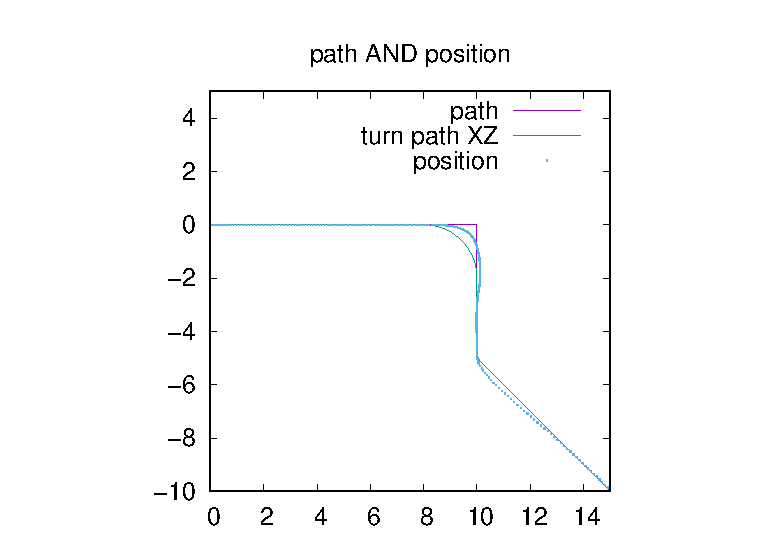
\includegraphics[width=90mm]{default_path_prokladka_position.eps}
		\end{figure}
\end{frame}

%--------------------------------------------------------------------------------
\section[Радиовещание]{Радиовещание}
\subsection[Радиовещание]{Радиовещание}
\begin{frame}
\frametitle{Радиовещание}
\small
\begin{figure}[ht!]
    \begin{tikzpicture}[>=latex]
        \draw[thick,dotted] (5,5)  rectangle  (1,3) ; %
				\node at (3,4) {Radio};
        \fill[red] (1,1) circle (2pt); % центр
        \draw[blue, ->]  (1,1) -- node[left=3pt] {$t_1$}  (1.5,3) ; % радиу
        \fill[red] (2.5,1) circle (2pt);
				\draw[blue, ->]  (2.5,1) -- node[left=3pt] {$t_2$}  (2.5,3) ;
				
				\fill[black] (3.5,1) circle (1pt);
				\fill[black] (3.7,1) circle (1pt);
				\fill[black] (3.9,1) circle (1pt);
				
        \fill[red] (5,1) circle (2pt);
				\draw[blue, ->]  (5,1) -- node[left=3pt] {$t_n$}  (4.5,3) ;
    \end{tikzpicture}
\end{figure}

$t_i$ - такт вещания текущей позиции.

\end{frame}
%--------------------------------------------------------------------------------
\section[Обнаружение конфликтов]{Обнаружение конфликтов}
\subsection[Этапы]{Этапы}
\begin{frame}
\frametitle{Этапы обнаружения конфликта}
\small


\begin{itemize}
	\item Проверка расстояния 
	\item Проверка сближения
	\item Вычисление промежутка конфликта
\end{itemize}

\end{frame}
%--------------------------------------------------------------------------------
\subsection[Проверка расстояния]{Проверка расстояния}
\begin{frame}
\frametitle{Проверка расстояния}
\small

\begin{figure}[ht!]
    \begin{tikzpicture}[>=latex]
        \draw[thick,dotted] (1,1) circle (2cm); % окружность
        \fill[blue] (1,1) circle (2pt); % центр
        \draw[blue, -]  (1,1) -- node[left=3pt] {$R$}  (1,3) ; % радиу
        \fill[red] (2,3) circle (2pt);
        \fill[red] (2,1.5) circle (2pt);
    \end{tikzpicture}
\end{figure}

$R$ - радиус фильтрации.
\end{frame}

%--------------------------------------------------------------------------------
\subsection[Проверка сближения]{Проверка сближения}
\begin{frame}
\frametitle{Проверка сближения}
\small

\begin{figure}[ht!]
    \begin{tikzpicture}[>=latex]
        \draw[thick,dotted] (1,1) circle (2cm); % окружность
        \fill[blue] (1,1) circle  (2pt); % ла 1
        \fill[red] (2,1.5) circle (2pt); % ла 2

        \coordinate [label=left:$p_1$] (A) at (1,1); % обозн точки ла 1
        \coordinate [label=right:$p_2$] (B) at (2,1.5); % обозн точки ла 2
        \coordinate [label=left:$v_1$] (A1) at (1,2);
        \coordinate [label=right:$v_2$] (B1) at (1.5,2);

        \draw [->] (A) -- (B);

        \draw [->,blue] (A) -- (A1);

        \draw [->,red] (B) -- (B1);

        \draw [->] (A1) -- (B1);
    \end{tikzpicture}
\end{figure}

$$(p_2 - p_1, v_2 - v_1 ) < 0,$$
где $p_1, p_2$ - точки позиций в пространстве первого и второго судна соответственно, 
$v_1, v_2$ - векторы скорости первого и второго судна соответственно.

\end{frame}

%--------------------------------------------------------------------------------
\subsection[Вычисление промежутка конфликта]{Вычисление промежутка конфликта}
\begin{frame}
\frametitle{Вычисление промежутка конфликта}
\small

\begin{align*}
    ||(x_1(t), z_1(t))^T - (x_2(t), z_2(t))^T|| &\leq R_{30},\\
    |y_1(t) - y_2(t)| &\leq H_{30},
\end{align*}

где $R_{30}$ --- радиус защитного объема, $H_{30}$ --- высота защитного объема. 

\end{frame}

%--------------------------------------------------------------------------------
\section[Заключение]{Заключение}
\subsection[Заключение]{Заключение}
\begin{frame}
\frametitle{Заключение}
\small

???

\end{frame}

%--------------------------------------------------------------------------------
\section[Заключение]{Заключение}
\subsection[Спасибо за внимание]{Спасибо за внимание}
\begin{frame}
\frametitle{Спасибо за внимание}
\small

???

\end{frame}



\end{document}